\documentclass{article}\usepackage[]{graphicx}\usepackage[]{xcolor}
% maxwidth is the original width if it is less than linewidth
% otherwise use linewidth (to make sure the graphics do not exceed the margin)
\makeatletter
\def\maxwidth{ %
  \ifdim\Gin@nat@width>\linewidth
    \linewidth
  \else
    \Gin@nat@width
  \fi
}
\makeatother

\definecolor{fgcolor}{rgb}{0.345, 0.345, 0.345}
\newcommand{\hlnum}[1]{\textcolor[rgb]{0.686,0.059,0.569}{#1}}%
\newcommand{\hlsng}[1]{\textcolor[rgb]{0.192,0.494,0.8}{#1}}%
\newcommand{\hlcom}[1]{\textcolor[rgb]{0.678,0.584,0.686}{\textit{#1}}}%
\newcommand{\hlopt}[1]{\textcolor[rgb]{0,0,0}{#1}}%
\newcommand{\hldef}[1]{\textcolor[rgb]{0.345,0.345,0.345}{#1}}%
\newcommand{\hlkwa}[1]{\textcolor[rgb]{0.161,0.373,0.58}{\textbf{#1}}}%
\newcommand{\hlkwb}[1]{\textcolor[rgb]{0.69,0.353,0.396}{#1}}%
\newcommand{\hlkwc}[1]{\textcolor[rgb]{0.333,0.667,0.333}{#1}}%
\newcommand{\hlkwd}[1]{\textcolor[rgb]{0.737,0.353,0.396}{\textbf{#1}}}%
\let\hlipl\hlkwb

\usepackage{framed}
\makeatletter
\newenvironment{kframe}{%
 \def\at@end@of@kframe{}%
 \ifinner\ifhmode%
  \def\at@end@of@kframe{\end{minipage}}%
  \begin{minipage}{\columnwidth}%
 \fi\fi%
 \def\FrameCommand##1{\hskip\@totalleftmargin \hskip-\fboxsep
 \colorbox{shadecolor}{##1}\hskip-\fboxsep
     % There is no \\@totalrightmargin, so:
     \hskip-\linewidth \hskip-\@totalleftmargin \hskip\columnwidth}%
 \MakeFramed {\advance\hsize-\width
   \@totalleftmargin\z@ \linewidth\hsize
   \@setminipage}}%
 {\par\unskip\endMakeFramed%
 \at@end@of@kframe}
\makeatother

\definecolor{shadecolor}{rgb}{.97, .97, .97}
\definecolor{messagecolor}{rgb}{0, 0, 0}
\definecolor{warningcolor}{rgb}{1, 0, 1}
\definecolor{errorcolor}{rgb}{1, 0, 0}
\newenvironment{knitrout}{}{} % an empty environment to be redefined in TeX

\usepackage{alltt}
\usepackage{amsmath} %This allows me to use the align functionality.
                     %If you find yourself trying to replicate
                     %something you found online, ensure you're
                     %loading the necessary packages!
\usepackage{amsfonts}%Math font
\usepackage{graphicx}%For including graphics
\usepackage{hyperref}%For Hyperlinks
\usepackage[shortlabels]{enumitem}% For enumerated lists with labels specified
                                  % We had to run tlmgr_install("enumitem") in R
\hypersetup{colorlinks = true,citecolor=black} %set citations to have black (not green) color
\usepackage{natbib}        %For the bibliography
\setlength{\bibsep}{0pt plus 0.3ex}
\bibliographystyle{apalike}%For the bibliography
\usepackage[margin=0.50in]{geometry}
\usepackage{float}
\usepackage{multicol}

%fix for figures
\usepackage{caption}
\newenvironment{Figure}
  {\par\medskip\noindent\minipage{\linewidth}}
  {\endminipage\par\medskip}
\IfFileExists{upquote.sty}{\usepackage{upquote}}{}
\begin{document}

\vspace{-1in}
\title{Lab 10 -- MATH 240 -- Computational Statistics}

\author{
  Charles Hooey \\
  Colgate University  \\
  Mathematical Economics Major  \\
  {\tt chooey@colgate.edu}
}

\date{}

\maketitle

\begin{multicols}{2}
%\raggedcolumns % If your spacing gets messed up try uncommenting 
                % this line
\begin{abstract}
This laboratory assignment aims to use \texttt{R} in order to understand how margins of error are calculated within Gallup polls. The first part of this assignment involved creating a basic simulation of the gallup data, which we would interact with graphically and through random re sampling to estimate the margin of error for the data. The graphical analysis conducted within this part led us to conclude that re sampling yields a more accurate estimate of margin of error than data simulation itself does. The second part of the assignment had us conduct many different simulations across varying sample sizes and probabilities. We first analyzed these simulations with our estimated margin of error, and then with the true margin of error, which led us to conclude that we may need to analyze a larger range of sample sizes in order to more accurately observe the relationship between margin of error and sample size.
\end{abstract}

\noindent \textbf{Keywords:} Resampling, Point Estimation, Margin of Error

\section{Introduction}
This assignment aimed to analyze the derivation of a margin of error from the Gallup poll, a poll conducted by Gallup which surveyed US citizens of their current satisfaction with the position of the United States. We wanted to determine how this margin of error was calculated, and how the variation of sample size may affect its accuracy. To accomplish this, we first plan to simulate data for the Gallup in order to approximate its probability distribution. We also want to re sample this data, which involves randomly selecting representative samples of the population data with replacement. By analyzing the range within the distributions of these data both graphically and numerically, we hope to estimate an approximate margin of error, and determine the most efficient method of doing so. Following such, we plan to analyze how varying sample size and probability will effect the calculation of margin of error by conducting many different simulations across specific ranges of $n$ and $p$. We also plan to use two different methods of calculating the margin of error for these simulations, comparing the differences and accuracy among each method.

\section{Simulating Data}
Within this laboratory assignment, we were tasked with determining how the government derives the margin of errors that they report within the gallop poll, a poll which asks US citizens whether they are satisfied or dissatisfied with the current state of the country. The first step towards better understanding this question was using R to conduct a simulation study. Using a specified probability value of 0.39 to generate a random binomial distribution for the data, we simulated 10000 gallop polls, each with the same population of 1000. Plotting this distribution with a histogram and density plot as seen in figure \ref{fig1} led to a conclusion that the simulated data is not skewed. Furthermore, the range between the distribution's middle 95 percent was approximately 100, meaning that this data had a margin of error close to $\pm 50$ percent. Comparing this with the $\pm 2$ percent reported by Gallup leads us to conclude that the conducted data simulation is not accurately representative of the population reported by Gallup.

\begin{Figure}
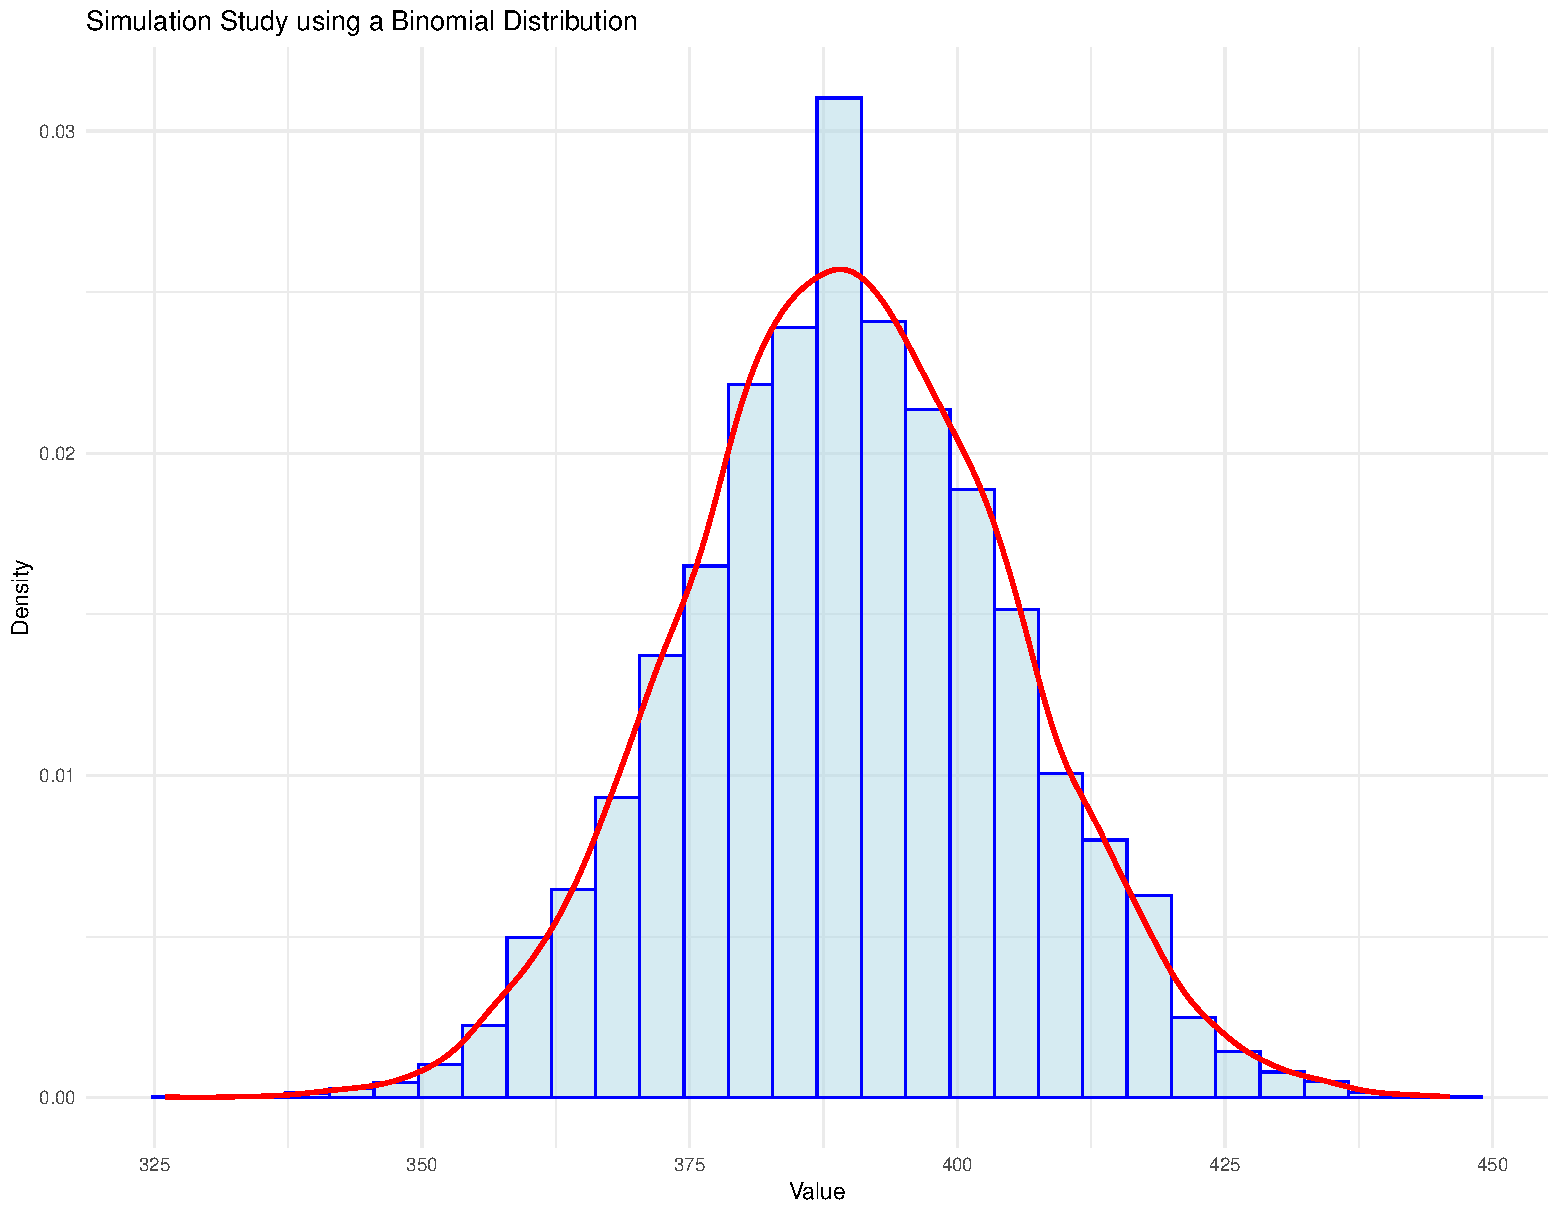
\includegraphics[scale=0.4]{Simplot.pdf}
\captionof{figure}{Histogram of Simulated Data}
\label{fig1}
\end{Figure}

\section{Resampling}
The second part of this laboratory assignment involved the use of resampling in order to approximate a probability distribution for the data reported by Gallup. This process involved using data collected within part one to retrieve 1000 random samples with replacement, with each being representative of the original population. We then plotted this data with a histogram and density plot as seen within figure \ref{fig2}, with the data once again not skewed. Furthermore, the range between the distribution's middle 95 percent was much smaller than that of our original data simulation at an approximate value of one, meaning the margin of error was approximately $\pm 0.5$ percent. This suggests that resampling allows us to more accurately approximate the unknown distribution of the Gallup Data than the conclusions offered by only conducting a simulation of the data.

\section{Simulation over n and p}
For the third part of this laboratory assignment we conducted the same analysis we had within part one, this time performing 10000 simulations for $n$ in $(100, 110, 120,...,3000)$ and $p$ in $(0.01, 0.02,...,0.99)$, with $n$ being the population size and $p$ the probability that an individual was satisfied with the state of the country as reported within the gallup poll. Our goal here was to record the approximate margin of error for each simulation by recording the middle 95 percent of the distribution's range, and interpret how this margin would fluctuate as $n$ and $p$ were shifted. We then visualized this data by using \texttt{ggplot} to create a \texttt{geom\_raster} plot, which as seen in figure \ref{fig3} plots the estimated margin of error as a function of $n$ and $p$ \citep{ggplot}. This figure suggests that margin of error peaks when at a probability value of $p = 0.5$, and consequently decreases going towards zero and 1.00. This may suggest that the data simulation will be less accurate if people are not as certain of their opinions of the country, which would cause the probability to grow closer to a value of 0.5 where the simulation is the least accurate. Furthermore, the margin of error decreases across the entire graph as our sample size increases, which is concurrent with our knowledge that a larger sample will be more accurately representative of the data.
\begin{Figure}
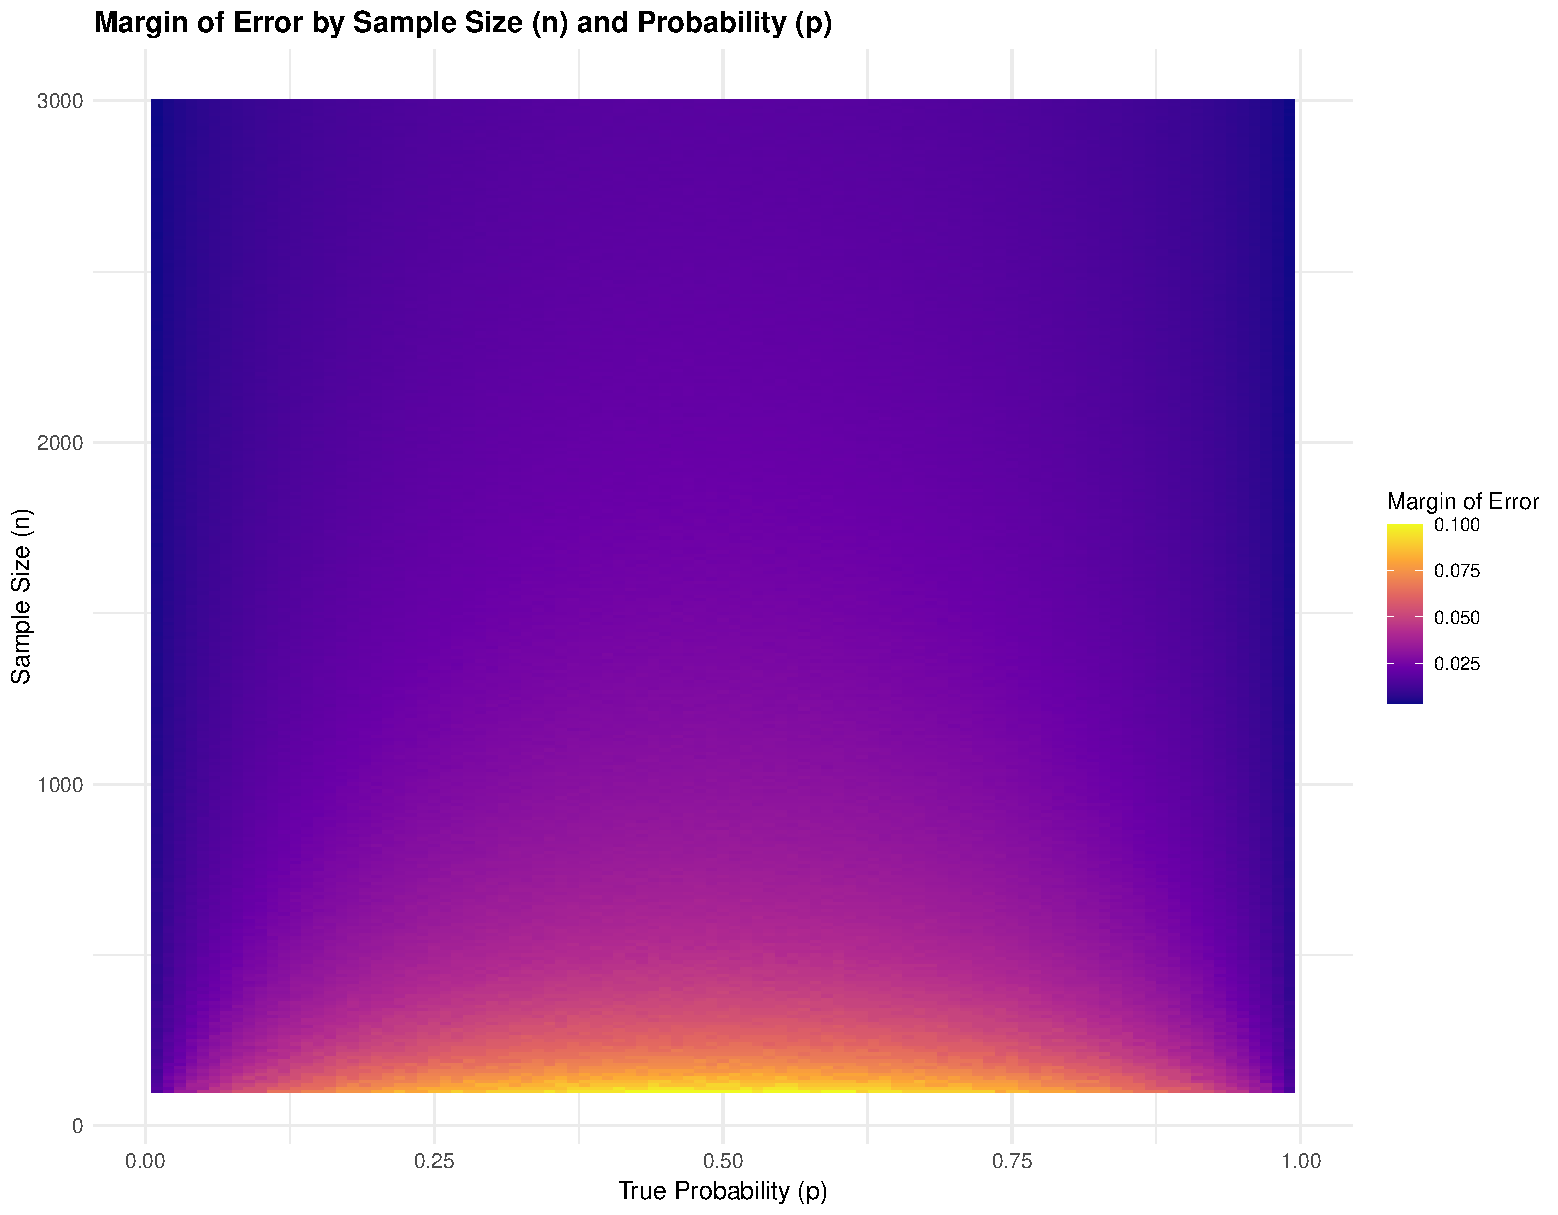
\includegraphics[scale=0.4]{pt3plot.pdf}
\captionof{figure}{Raster Plot of Estimated Margin of Error as a function of n and p}
\label{fig3}
\end{Figure}
\section{Calculating the Actual Margin of Error}
The final part of this laboratory assignment had us conduct the same simulation we had within part three, though this time using the Wilson margin of error formula. This formula would calculate the actual margin of error, rather than approximate it such as we had by halving the middle 95 percent of the data's distribution. After collecting the simulation data, we visualized it by creating another raster plot, as seen within figure \ref{fig4}. This figure is concurrent with the assumption made in part three regarding the margin of error increasing as $p$ approaches a value of 0.50, but differs from figure \ref{fig3} in that we do not observe any discernible effect on the margin of error from the sample size ($n$). This could suggest that the sample size of our data is inaccurate and is not large enough to accurately approximate the actual population of individuals reported by Gallup. In order to get a more accurate approximation of how $n$ effects the Wilson margin of error I would conduct this simulation over a larger range of sample sizes, and observe whether a discernible difference in the data's margin of error emerges from a larger sample size.
\begin{Figure}
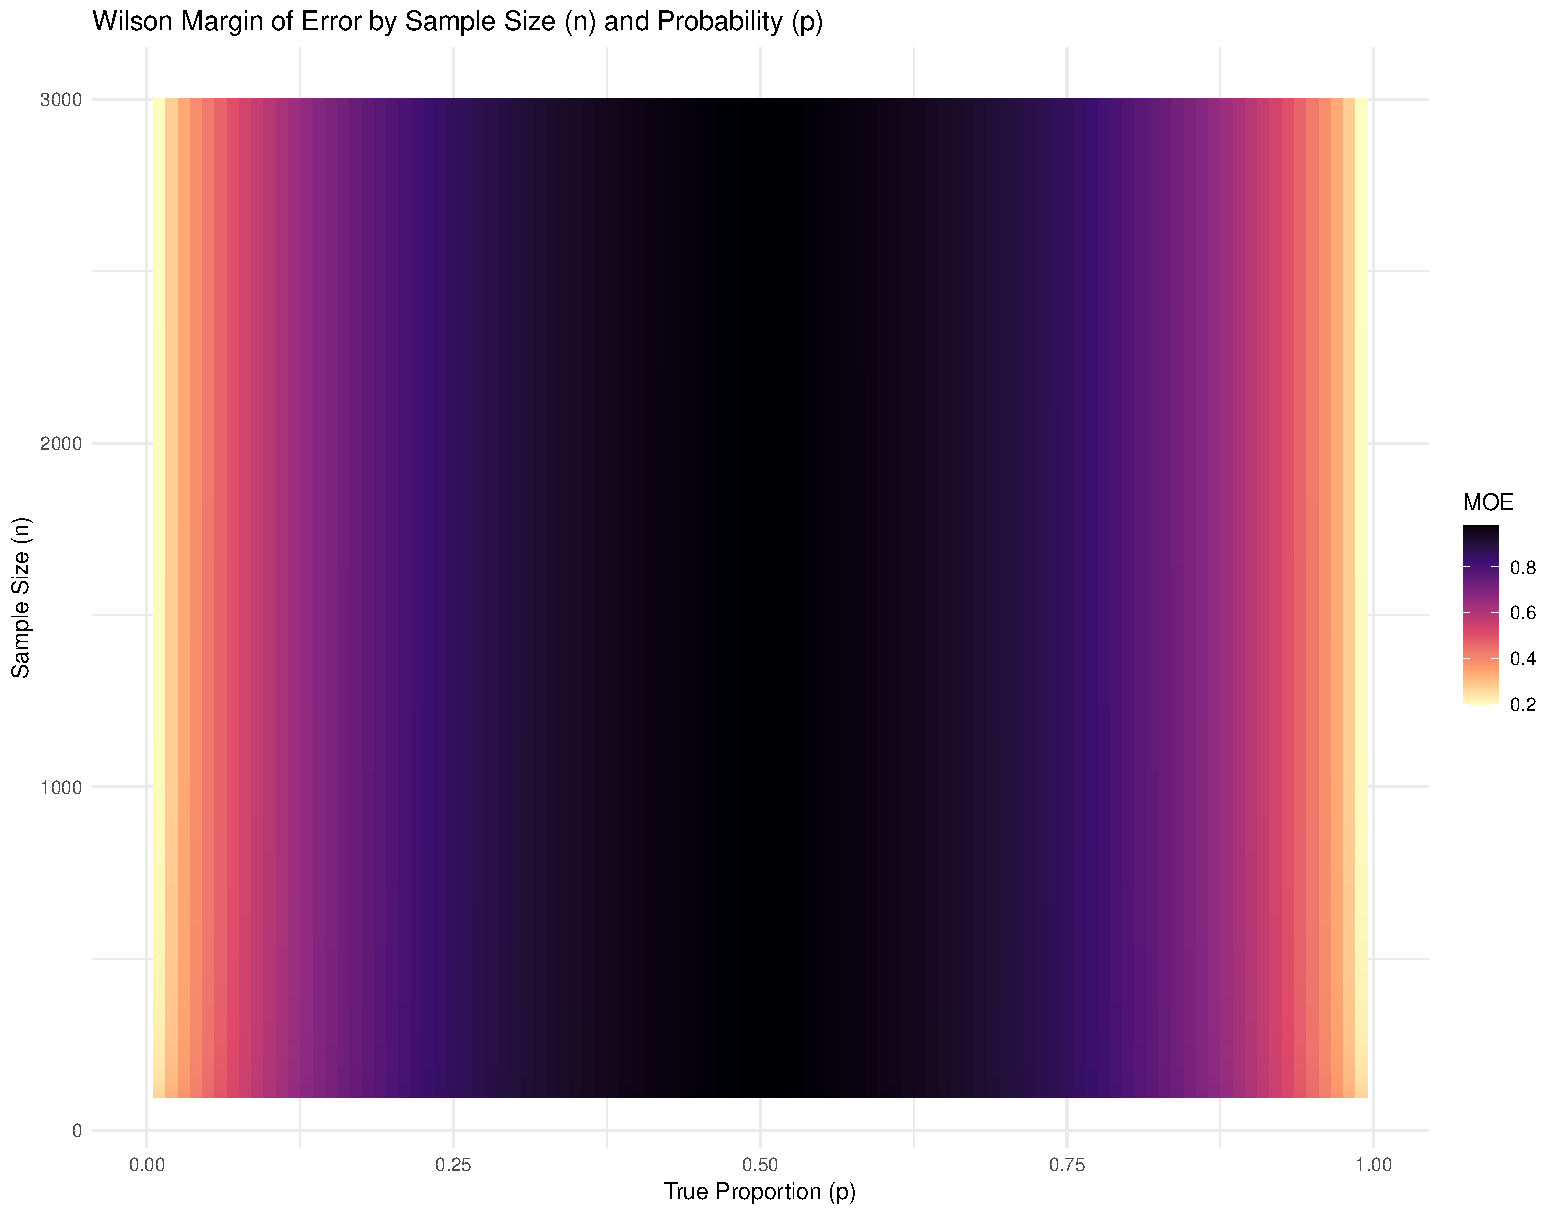
\includegraphics[scale=0.4]{pt4plot.pdf}
\captionof{figure}{Raster Plot of True Margin of Error as a function of n and p}
\label{fig4}
\end{Figure}
%%%%%%%%%%%%%%%%%%%%%%%%%%%%%%%%%%%%%%%%%%%%%%%%%%%%%%%%%%%%%%%%%%%%%%%%%%%%%%%%
% Bibliography
%%%%%%%%%%%%%%%%%%%%%%%%%%%%%%%%%%%%%%%%%%%%%%%%%%%%%%%%%%%%%%%%%%%%%%%%%%%%%%%%
\vspace{2em}

\noindent\textbf{Bibliography:} 

\begin{tiny}
\bibliography{bib}
\end{tiny}
\end{multicols}

%%%%%%%%%%%%%%%%%%%%%%%%%%%%%%%%%%%%%%%%%%%%%%%%%%%%%%%%%%%%%%%%%%%%%%%%%%%%%%%%
% Appendix
%%%%%%%%%%%%%%%%%%%%%%%%%%%%%%%%%%%%%%%%%%%%%%%%%%%%%%%%%%%%%%%%%%%%%%%%%%%%%%%%
\newpage
\onecolumn
\section{Appendix}

\begin{Figure}
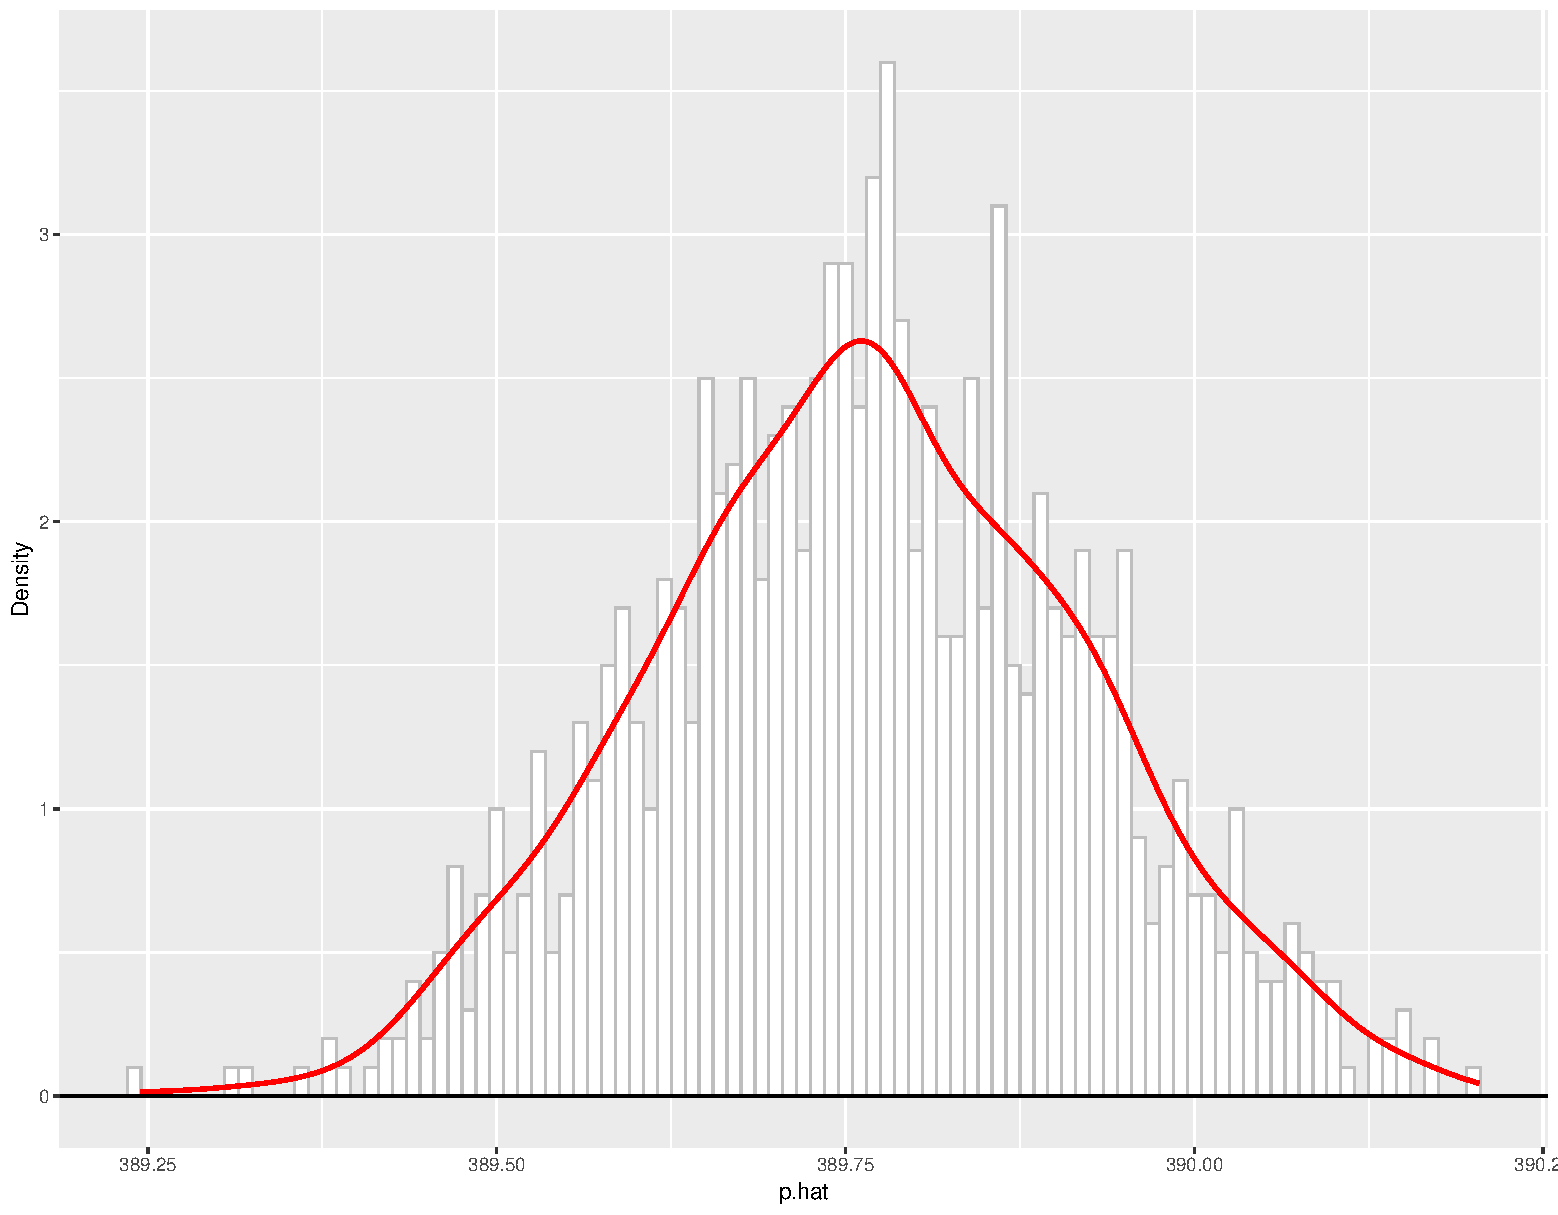
\includegraphics[scale=0.4]{resampleplot.pdf}
\captionof{figure}{Histogram of Resampled Data}
\label{fig2}
\end{Figure}

\end{document}
